\documentclass[a4paper,12pt,obeyspaces,spaces,hyphens]{article}

\def \trainingtype{onsite}
\def \agendalanguage{french}

\input{agenda/debugging.inc}

\usepackage{agenda}

\begin{document}

\feshowtitle

\feagendasummaryitem{Titre}{
  {\bf \trainingtitle{}}
}
\feagendasummaryitem{Objectifs\newline opérationnels}{
  \traininggoals{}
}
\feagendasummaryitem{Durée}{
  \feshowduration{}
}
\onsitepedagogics{40}{60}
\feagendasummaryitem{Formateur}{
  Clément Léger
  \newline \url{https://bootlin.com/company/staff/clement-leger/}
}
\feagendasummaryitem{Langue}{
  \traininglanguages{}
}
\feagendasummaryitem{Public visé}{
  \trainingaudience{}
}
\feagendasummaryitem{Pré-requis}{
  \trainingprerequisites{}
}
\ferequiredequipmentonsite{22.04}
\certificate{}
\disabilities{}

\feagendatwocolumn
{Matériel utilisé pour les travaux pratiques}
{
  Une de ces cartes de STMicroelectronics: {\bf
  STM32MP157A-DK1}, {\bf STM32MP157D-DK1}, {\bf STM32MP157C-DK2} ou
  {\bf STM32MP157F-DK2}
  \begin{itemize}
  \item Processeur STM32MP157, double Cortex-A7, de STMicroelectronics
  \item Alimentée par USB
  \item 512 Mo DDR3L RAM
  \item Port Gigabit Ethernet port
  \item 4 ports hôte USB 2.0
  \item 1 port USB-C OTG
  \item 1 connecteur Micro SD
  \item Debugger ST-LINK/V2-1 sur la carte
  \item Connecteurs compatibles Arduino Uno v3
  \item Codec audio
  \item Divers: boutons, LEDs
  \item Écran LCD tactile (uniquement sur cartes DK2)
  \end{itemize}
}{}
{
  \begin{center}
    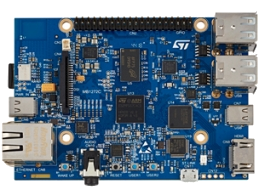
\includegraphics[width=5cm]{../slides/discovery-board-dk1/discovery-board-dk1.png}
  \end{center}
}

\section{1\textsuperscript{er} Jour - Matin}

\feagendaonecolumn
{Cours - Pile logicielle Linux}
{
  \begin{itemize}
  \item Vue d'ensemble: comprendre l'architecture général d'un système
    Linux, aperçu des principaux composants
  \item Différence entre un processus et un thread, comment les
    applications fonctionnent de façon concurrente.
  \item Fichiers ELF et outils d'analyse associés.
  \item Organisation de l'espace d'adressage des applications: heap,
    stack, bibliothèques partagées, etc.
  \item MMU et gestion mémoire: espaces d'adressage physique et
    virtuel
  \item Contexte d'exécution dans le noyau: threads noyau, workqueues,
    interruptions, interruptions threadées, softirq
  \end{itemize}
}

\feagendaonecolumn
{Cours - Outils usuels d'analyse et d'observation}
{
  \begin{itemize}
  \item Analyse d'un binaire ELF avec les outils GNU ({\em objdump},
    {\em addr2line})
  \item Outils pour monitorer un système Linux: processus,
    consommation et mapping mémoire, ressources
  \item Utilisation de {\em vmstat}, {\em iostat}, {\em ps}, {\em
      top}, {\em iotop}, {\em free} et compréhension des métriques
    qu'ils fournissent.
  \item Systèmes de fichiers virtuels: {\em procfs}, {\em sysfs} et
    {\em debugfs}
  \end{itemize}
}

\section{1\textsuperscript{er} Jour - Après-midi}

\feagendaonecolumn
{Démo - Comprendre ce qui fonctionne sur un système et sa charge}
{
  \begin{itemize}
  \item Observation des processus en cours d'exécution avec {\em ps} et {\em top}
  \item Observation des mappings mémoire avec {\em procfs} et {\em pmap}
  \item Monitoring d'aurtres ressources avec {\em iostat}, {\em
      vmstat} et {\em netstat}
 \end{itemize}
}

\feagendatwocolumn
{Cours - Debug d'une application}
{
  \begin{itemize}
  \item Utilisation de {\em gdb} sur un processus en cours d'exécution.
  \item Comprendre l'impact des optimisations du compilateur sur la
    capacité à débugger un programme.
  \item Analyse post-mortem avec des fichiers {\em core}
  \item Debug à distance avec {\em gdbserver}.
  \item Étendre les capacités de {\em gdb} en utilisant des scripts
    Python.
  \end{itemize}
}
{Démo - Résoudre un crash applicatif}
{
  \begin{itemize}
  \item Analyse d'un code C compilé avec \code{compiler-explorer} pour
    comprendre les optimisations.
  \item Utilisation de {\em gdb} en ligne de commande, puis depuis un
    IDE.
  \item Utilisation des possibilités de scripting Python dans {\em gdb}.
  \item Debugger une application {\em post mortem} avec un {\em core
      dump} et {\em gdb}
  \end{itemize}
}

\section{2\textsuperscript{ème} Jour - Matin}

\feagendatwocolumn
{Cours - Tracing d'une application}
{
  \begin{itemize}
  \item Tracing des appels systèmes avec {\em strace}.
  \item Tracing des appels à des bibliothèques partagées avec {\em ltrace}.
  \end{itemize}
}
{Démo – Débugger des problèmes applicatifs}
{
  \begin{itemize}
  \item Analyser les appels à des bibliothèques partagées d'une
    application en utilisant {\em ltrace}.
  \item Débugger une application qui fonctionne de manière incorrecte
    en utilisant {\em strace}.
  \end{itemize}
}

\feagendatwocolumn
{Cours - Problèmes liés à la mémoire}
{
  \begin{itemize}
  \item Problèmes classiques liés à la mémoire: {\em buffer overflow},
    {\em segmentation fault}, fuite mémoire, collision pile/tas.
  \item Outils de détection/investigation de problèmes mémoires: {\em
      valgrind}, {\em libefence}, etc.
  \item Profiling de l'utilisation du tas en utilisant {\em Massif}
  \end{itemize}
}
{Démo – Débugger des problèmes liés à la mémoire}
{
  \begin{itemize}
  \item Fuites mémoire et détection de comportement incorrects avec
    {\em valgrind} et {\em vgdb}.
  \item Problèmes de performance liés à une sur-allocation.
  \item Visualisation de l'utilisation du tas par une application en
    utilisant {\em Massif}.
  \end{itemize}
}

\section{2\textsuperscript{ème} Jour - Après-midi}

\feagendatwocolumn
{Cours – Profiling d'application}
{
  \begin{itemize}
  \item Problèmes de performance.
  \item Récupération d'informations de profiling avec {\em perf}.
  \item Analyse du graphe d'appel d'une application avec {\em
      Callgrind} et {\em KCachegrind}.
  \item Filtrage du jeu de données récupéré.
  \item Interprétation, des données enregistrées avec {\em perf}.
  \end{itemize}
}
{Démo - Profiling d'application}
{
  \begin{itemize}
  \item Profiling d'une application avec {\em Callgrind}/{\em
      KCachegrind}.
  \item Analyse des performances d'une application avec {\em perf}.
  \item Générer un {\em flamegraph} avec {\em FlameGraph}.
  \end{itemize}
}

\section{3\textsuperscript{ème} Jour - Matin}

\feagendatwocolumn
{Cours - Profiling et tracing de l'ensemble du système}
{
  \begin{itemize}
  \item Profiling du système complet avec {\em perf}.
  \item Utilisation de {\em kprobes} pour ajouter des points de trace
    supplémentaires sans recompilation
  \item Outils {\em eBPF} ({\em bcctools}, {\em bpftrace}, etc) pour
    les scénarios de tracing complexes.
  \item Tracing d'application et du noyau et visualisation des traces
    avec {\em ftrace}, {\em kernelshark} ou {\em LTTng}
  \end{itemize}
}
{Démo - Profiling et tracing de l'ensemble du système}
{
  \begin{itemize}
  \item Profiling du système complet avec {\em perf}.
  \item Latence d'interruptions avec {\em ftrace}.
  \item Tracing et visualisation de l'activité du système avec {\em
      kernelshark} ou {\em LTTng}
  \end{itemize}
}

\section{3\textsuperscript{ème} Jour - Après-midi}

\feagendatwocolumn
{Cours - Debugging du noyau Linux}
{
  \begin{itemize}
  \item Sorties de la compilation du noyau Linux utiles pour le
    debugging (\code{vmlinux}, \code{System.map}).
  \item Comprendre et configurer le comportement des {\em kernel oops}.
  \item Analyse post-mortem d'un crash kernel avec {\em crash}.
  \item Problèmes mémoire au niveau kernel ({\em KASAN}, {\em UBSAN}, {\em Kmemleak}).
  \item Debugging du noyau Linux avec {\em KGDB} et {\em KDB}.
  \item Options du noyau Linux pour le debug des problèmes de verrous
    (lockdep)
  \item Autres options de configuration du noyau Linux utiles pour le
    debug.
  \end{itemize}
}
{Démo - Debugging du noyau Linux}
{
  \begin{itemize}
  \item Analyse d'un {\em oops} après utilisation d'un module noyau
    incorrect, avec {\em obdjump} et {\em addr2line}.
  \item Debugging d'un {\em deadlock} avec les options {\em PROVE\_LOCKING}.
  \item Détecter un {\em undefined behavior} avec {\em UBSAN} dans le noyau Linux.
  \item Trouver une fuite mémoire avec {\em kmemleak}.
  \item Débugger un module noyau avec {\em KGDB}.
  \end{itemize}
}

\end{document}

